% Main document of the project, this will include all the other parts involving the documentation...

\documentclass[a4paper]{article}
\usepackage[utf8]{inputenc}
\usepackage[T1]{fontenc}

%% Sets page size and margins
\usepackage[a4paper,top=3cm,bottom=2cm,left=3cm,right=3cm,marginparwidth=1.75cm]{geometry}

%% Useful packages
\usepackage[table,xcdraw]{xcolor}
\usepackage{longtable}
\usepackage{amsmath}
\usepackage{floatrow}
\usepackage{graphicx}
\graphicspath{ {./images/} }
\usepackage[colorinlistoftodos]{todonotes}
\usepackage[colorlinks=true, allcolors=blue]{hyperref}
\usepackage{amsmath}
\usepackage{chngcntr}
\usepackage{wrapfig}
\usepackage{eurosym}
\usepackage{caption}
\usepackage{subcaption}
\usepackage{listings}
\usepackage{placeins}
\usepackage{multicol}
\usepackage{verbatim}
\usepackage{csvsimple}
\usepackage{listings}
\usepackage[spanish]{babel}
\renewcommand\spanishtablename{Tabla}
\selectlanguage{spanish}
\usepackage{colortbl}
\usepackage{cite}
\usepackage{xr}

\usepackage[toc,page]{appendix}
\usepackage{pdflscape}

\expandafter\def\expandafter\appendixpagename%
\expandafter{\expandafter\Huge\appendixpagename}

\usepackage{afterpage}

\addto\captionsspanish{%
  \renewcommand\appendixname{\Huge Apéndices}
  \renewcommand\appendixpagename{\Huge Apéndices}
}

\captionsetup[table]{position=bottom}

\renewcommand{\lstlistingname}{Código}% 
\renewcommand{\lstlistlistingname}{Lista de código}% List of Listings -> List of Algorithms

% extracted from internet: https://timmurphy.org/2014/01/27/displaying-code-in-latex-documents/
\definecolor{lbcolor}{rgb}{0.93,0.93,0.93}
\lstset{  
    frame=tb, % draw a frame at the top and bottom of the code block
    tabsize=4, % tab space width
    showstringspaces=false, % don't mark spaces in strings
    numbers=left, % display line numbers on the left
    commentstyle=\color{green}, % comment color
    keywordstyle=\color{blue}, % keyword color
    stringstyle=\color{red},
    backgroundcolor=\color{lbcolor}
}

\definecolor{main-color}{rgb}{0.6627, 0.7176, 0.7764}
\definecolor{back-color}{rgb}{0.1686, 0.1686, 0.1686}
\definecolor{string-color}{rgb}{0.3333, 0.5254, 0.345}
\definecolor{key-color}{rgb}{0.8, 0.47, 0.196}
\lstdefinestyle{idlstyle}
{
    language = C++,
    keywordstyle = {\color{key-color}},
    keywordstyle = [3]{\color{blue}},
    otherkeywords = {in, int ,interface, out, inout},
    morekeywords = [3]{in, out, inout}
}

\setcounter{secnumdepth}{3}
\setcounter{tocdepth}{3}

% \title{Integrating COMPSs and OmpSs Programming Models to support distributed heterogeneous computing environments}
\title{Integrating COMPSs and OmpSs Programming Models to support distributed heterogeneous computing environments}
\author
{
Marc Domínguez de la Rocha
\and
Rosa M. Badia
\and
Jorge Ejarque
}

\date{Abril 2019}

\begin{document}

\maketitle

\newpage
\renewcommand{\contentsname}{Índice}
\tableofcontents
\newpage

%GEP

La sección que continúa es relativa a la gestión del proyecto y se mantiene dentro del trabajo porque corresponde al estado del arte. El resto de secciones que conforman la gestión del proyecto se encuentran en los apéndices \ref{sec:sostenibilidad} \ref{sec:planificacion}

% La siguiente seccion enmarca el contexto
% que envuelve al proyecto y de alguna
% manera el por qué
\section{Contexto}

Hoy en día se tiende a tener distintos recursos de cómputo en un solo dispositivo, por ejemplo, en un teléfono móvil ya tenemos al menos un procesador y una tarjeta gráfica, pero no tan sólo en el ámbito más cotidiano (aunque no nos demos cuenta), sino que en los más profesionales y especializados está siendo también cada vez más común la heterogeneidad de los recursos de computación. 
\par\bigskip

El proyecto pretende facilitar la gestión de estos recursos de computación en entornos distribuidos, brindando un método robusto y eficiente para programar aplicaciones en estos entornos.
%Quienes son los actores? Quien se beneficia?


\subsection{Introducción}

Este proyecto es un Trabajo de Fin de Grado del Grado en Ingeniería Informática, especializado en el área de Ingeniería de Computadores. El grado es impartido por la \textit{Facultat d'Informàtica de Barcelona (FIB)} centro perteneciente a la \textit{Universitat Politècnica de Catalunya (UPC)}. 
\par\bigskip

El proyecto se desarrollará conjuntamente con el \textit{Barcelona Supercomputing Center (BSC)}, estudiaremos como podemos integrar los modelos de programación \textit{COMPSs} y \textit{OmpSs} para alcanzar este objetivo, implementaremos un prototipo y evaluaremos su rendimiento y características deseadas. 
%Indagar en cuales son estas caracteristicas? 

\subsection{Actores}

Los actores en este proyecto serán las personas que tomen parte en él, ya sea de manera directa o indirecta. Con esto quiero decir, que tanto las personas que tomen parte en el desarrollo \textit{per se} como las personas que se nutran de este, serán los actores.

\begin{itemize}
 \item \textbf{Desarrollador:} La figura del desarrollador \textbf{debe} ser la persona que trabaje de manera más directa en el proyecto. En este proyecto únicamente habrá un desarrollador que ha elaborado la documentación que leerás a continuación y dará forma a los objetivos tangibles del proyecto.  
 \item \textbf{Director y codirector:} Pese a que el desarrollador tendrá el papel principal en el proyecto, el director y el codirector le guiarán en el camino abierto que es el desarrollo del proyecto. Se establecerán reuniones de seguimiento donde serán capaces de hacer un correcto supervisamiento de las actividades propuestas para el proyecto.
 \item \textbf{Barcelona Supercomputing Center:} De manera directa el centro otorga al desarrollador un lugar de trabajo y un equipo informático. Por otra parte, cuenta con el soporte por parte de los equipos de desarrollo de \textit{COMPSs} (del cual forma parte el desarrollador) y de \textit{OmpSs} para cualquier incidencia relacionada con su \textit{software} y derivados.
 \item \textbf{Beneficiarios:} \textit{COMPSs} es utilizado para proyectos europeos en los cuales el \textit{BSC} toma parte, el proyecto podrá ser útil para algunos de ellos, además todo departamento del \textit{BSC} que utilice \textit{COMPSs} para el desarrollo de aplicaciones podrá utilizarlo.
\end{itemize}

\section{Estado del arte}

%check si te estas patillando lo de ``centenares''
Existen centenares de modelos de programación, véanse \textit{OpenMP}, \textit{OmpSs}, \textit{MPI}, \textit{COMPSs} y un largo etcétera. De alguna manera el objetivo en común fue y es aprovechar los cada vez más abundantes recursos en las máquinas, que finalmente no sólo han crecido en abundancia si no en diversidad. La filosofía sigue siendo la misma, sacar el mayor rendimiento posible a nuestras máquinas. 
\par\bigskip

Para esto son necesarios modelos de programación que nos den la posibilidad de utilizar los recursos y nos ayuden a explotar la posible sinergia entre estos en ciertas aplicaciones. 
\par\bigskip

La diferencia más elemental entre los modelos, es en como se gestiona la memoria, o bien como la memoria está dispuesta en el modelo. Con \textit{shared memory} (\textit{OpenMP}, \textit{OmpSs}...), se aprovecha que el conjunto de hilos de ejecución (\textit{threads}) comparten la memoria, con \textit{distributed memory} (\textit{MPI}...) que se utilizan diferentes procesos con la posibilidad de que estos estén distribuidos entre distintos nodos, existen también modelos como \textit{CUDA} y \textit{OpenCL} que transfieren memoria de la \textit{CPU} a la memoria del acelerador en cuestión.
\par\bigskip

La integración de los modelos propuestos \textit{COMPSs} y \textit{OmpSs} nos otorgará la posibilidad de utilizar todos los recursos de la máquina, a continuación se ahonda en las características de ambos.

\subsection{COMPSs}

\textit{COMPSs} es desarrollado por el grupo \textit{Workflows and Distributed Computing} que pertenece al departamento de \textit{CS - Computer Science}.
\par\bigskip

\textit{COMPSs} es un modelo de programación para entornos distribuidos basado en la generación de tareas, el objetivo es hacer más sencilla la programación de aplicaciones y su ejecución en entornos distribuidos (clústers y \textit{clouds}, por ejemplo)\cite{badia2015comp}.La generación de tareas la efectua un programa principal ejecutado en secuencial, las tareas se especifican mediante la anotación de las funciones que se deseen, en tiempo de ejecución se genera un grafo de tareas y se detectan las dependencias entre estas para ejecutarlas en el orden correcto. Dado que está preparado para ejecutarse en entornos distribuidos también se detecta cuando son necesarias transferencias entre nodos.   \par\bigskip

Para facilitar más aún el uso del modelo, está dotado de un sistema de \textit{runtime} compuesto por un \textit{master} y un conjunto de \textit{workers}, el \textit{runtime} coexiste con la aplicación. Se encarga de detectar las dependencias que puedan surgir entre las tareas que genera el programa principal y las ejecuta a medida que las dependencias se resuelven. 
%\par\bigskip

\subsubsection{Modelo de programación} 
\label{compss_pm}

El \textit{runtime} de \textit{COMPSs} está implementado en \textit{Java} por lo cuál se soporta dicho lenguaje, además se desarrollaron los \textit{bindings} de \textit{Python}\cite{tejedor2017pycompss} y \textit{C/C++} para facilitar el portaje de aplicaciones en estos lenguajes a \textit{COMPSs}. 
\par\bigskip

Dicho esto, centraremos nuestros esfuerzos en \textit{C} y \textit{C++}. Para desarrollar una aplicación de \textit{COMPSs} en \textit{C/C++} necesitamos el programa principal (ejecutado en secuencial), una interfaz que especificará las funciones que \textit{a posteriori} serán tareas, y el código que realmente implementan estas tareas. 
\par\bigskip

Veamos en orden de enumeración ejemplos de los componentes de una aplicación.

%EJEMPLO INTERFACE
\begin{lstlisting}[caption={Interfaz de la aplicación 'ejemplo'.},captionpos=b, label={lst:ejemplo.idl}, style=idlstyle]
interface ejemplo {
    void funcionEjemplo(in int a, out int[a] array_a);
};
\end{lstlisting}

La interfaz de la imagen superior define una función llamada funcionEjemplo con un parámetro de entrada y uno de salida, las palabras clave \textit{in} y \textit{out} respectivamente otorgan estas propiedades a los parámetros, también se puede combinar con \textit{inout}. Cualquier llamada a la función será ejecutada como tarea.\smallskip

%EJEMPLO MASTER CODE
\begin{lstlisting}[caption={Fracción del código del programa principal}, captionpos=b, label={lst:ejemplo.cc}, language=C++]
    compss_on();

    int a = 10;
    int* array_a;

    funcionEjemplo(a, array_a);

    compss_wait_on(array_a);

    compss_off();
\end{lstlisting}

Esta imagen muestra el código del programa principal de manera reducida. Es tan sencillo como prometía, encendemos el \textit{runtime} de \textit{COMPSs}, preparamos los parámetros de la función, ejecutamos y finalmente esperamos a los parámetros de salida y apagamos el \textit{runtime}. \smallskip

\begin{lstlisting}[caption={Implementación de la función 'funcionEjemplo'}, captionpos=b, label={lst:ejemplo-functions.cc}, language=C++]
void funcionEjemplo(int a, int array_a[]) {
    for (int i = 0; i < a; ++i) {
        array_a[i] = a;
    }
}
\end{lstlisting}

Las tareas se implementan como funciones que serán ejecutadas por los workers. Salvo convenciones en los nombres de los ficheros para hacer la compilación de la aplicación esto es todo lo necesario para desarrollar una aplicación en \textit{COMPSs} de \textit{C/C++}.

\begin{comment}
\subsubsection{Compilación}

Para compilar la aplicacion en \textit{COMPSs} de \textit{C/C++}, 

\begin{figure}[H]
    \centering
    \caption{Proceso de compilado de una aplicación COMPSs C/C++}
%    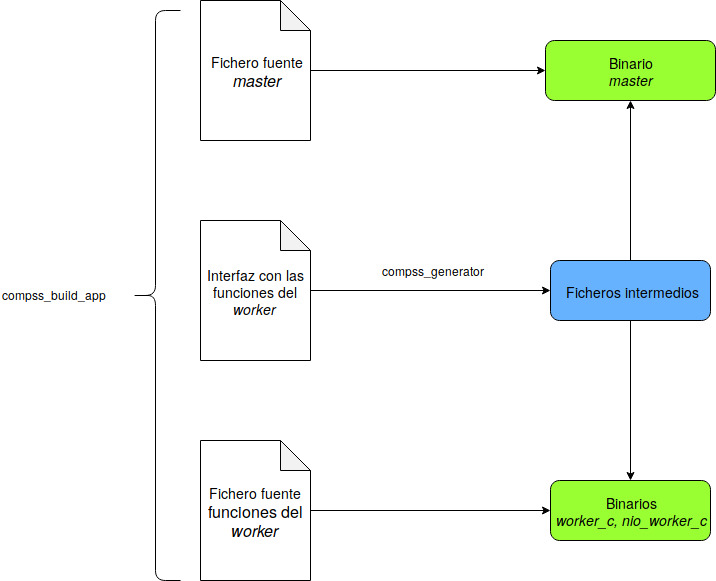
\includegraphics[width=\textwidth]{proceso_compilado.jpg}
    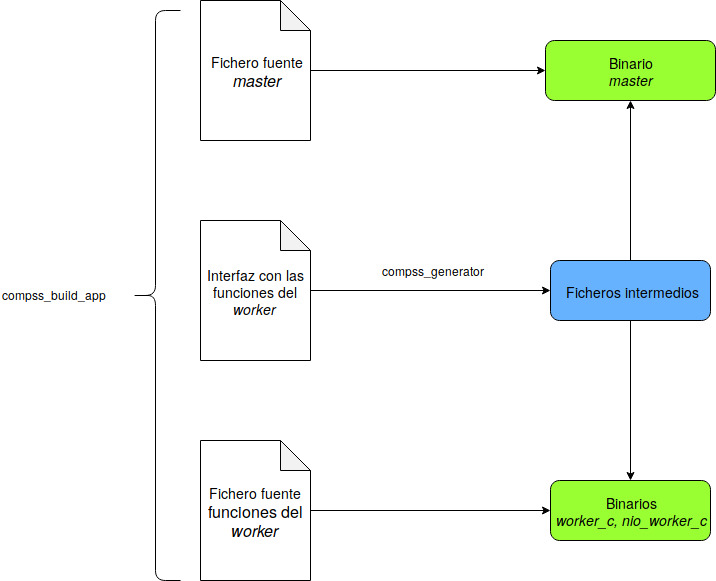
\includegraphics[scale=0.5]{proceso_compilado.jpg}
    \label{fig:proceso_compilado}
\end{figure}
\end{comment}

\subsubsection{Modelo de ejecución\label{modeloejecucion}}

El modelo de ejecución es sencillo, muy similar al modelo \textit{thread-pool}, al iniciar el \textit{runtime} se levanta el \textit{master} y un conjunto de \textit{workers}, a medida que se vayan generando tareas se estudiará qué \textit{workers} están libres y si cumplen los requisitos para ejecutar dicha tarea, y en ese caso la ejecutarán. 

\begin{figure}[H]
    \centering 
    \caption{Modelo de ejecución, basado en la aplicación 'ejemplo'.}
    %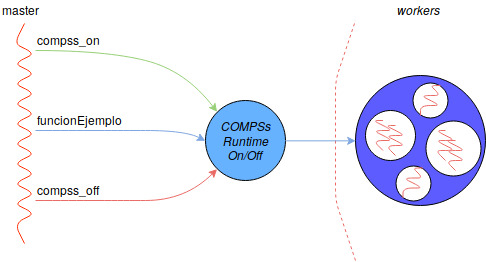
\includegraphics[width=\textwidth]{sta-masterworker.jpg}
    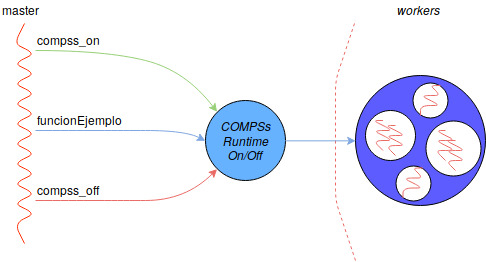
\includegraphics[scale=0.75]{sta-masterworker.jpg}
    \label{fig:masterworker_pool}
\end{figure}

La imagen muestra lo que sucede al ejecutar la aplicación de ejemplo de la sección \ref{compss_pm}, las líneas rojas curvas indican procesos (o bien \textit{threads}), lo importante sucede entre las flechas etiquetadas como compss\_on y compss\_off, la ejecución de la tarea. Se pide ejecutar la tarea funcionEjemplo al \textit{runtime} de \textit{COMPSs} y se decide en qué \textit{worker} se ejecutará. Hasta aquí podríamos pensar que es indéntico al \textit{thread-pool}. Nótese, que esto no es así, por el hecho de que no tenemos por qué hablar de una misma máquina, sino que pueden ser máquinas distintas, como se puede ver en el grupo de ordenadores de la imagen. 
\par\bigskip

En \textit{C/C++} existen dos tipos de \textit{worker}, uno \textbf{no persistente} y otro \textbf{persistente}. 

\begin{itemize}
 \item \textbf{No persistente:} Para cada tarea que se quiere ejecutar en uno de estos workers se debe crear el \textit{thread} y unas \textit{pipes} para hacer \textit{Inter-process communication} (IPC). %No sé si indagar en qué se pasa por las pipes, hmmm... qué se pasa por las pipes?
 \item \textbf{Persistente:} Este tipo de \textit{worker} se levanta una vez al inicio de la aplicación y espera recibir las tareas a ejecutar.
\end{itemize}


\subsection{OmpSs}

\textit{OmpSs} es desarrollado por el grupo \textit{PM - Programming Models}, perteneciente también al departamento de \textit{CS - Computer Science}.
\par\bigskip

\textit{OmpSs} es un modelo de programación que intenta explotar el paralelismo de las aplicaciones de una manera sencilla y aprovechando al máximo los recursos de la máquina\cite{duran2011ompss}. 
\par\bigskip
El nombre del modelo proviene de \textit{OpenMP} y \textit{StarSs} (modelo que desarrolló el \textit{BSC}), este integra funcionalidades presentes en ambos. Por parte de \textit{OpenMP} se quiere tomar la facilidad de paralelizar una aplicación secuencial insertando pragmas, y de \textit{StarSs} el modelo de ejecución basado en un \textit{thread-pool} y que permite la ejecución de código en más recursos que únicamente el procesador, es decir, que ofrece fácil gestión del resto de recursos de cómputo (\textit{GPUs}, \textit{FPGAs}, ...)\cite{sainz2014leveraging}\cite{filgueras2013heterogeneous}.

\subsubsection{Modelo de programación y ejecución}

El modelo de programación de \textit{OmpSs} se basa en la generación de tareas sencillamente insertando pragmas en código secuencial y a su vez facilitando la gestión de recursos heterogéneos. Veamos un pequeño ejemplo que muestre estas facultades.

\begin{lstlisting}[caption={Multiplicación de un bloque de una matriz utilizando GPUs.}, captionpos=b, label={lst:ompssmatmul.cc}, style=JStyle]
for (int i = 0; i < N; ++i) {
    for (int j = 0; j < N; ++j) {
        for (int k = 0; k < N; ++k) {
            #pragma omp target device(cuda) \
                               copy_deps    \
                               ndrange(2,N,N,32,32)
            #pragma omp task inout([N*N]C) in([N*N]A, [N*N]B)
            multiply_partitions_GPU(A[i*N+k], 
                                    B[k*N+j], 
                                    C[i*N+j], 
                                    n);
        }
    }
}
\end{lstlisting}

El código muestra una multiplicación de matrices por bloques. Con el primer pragma se indica que el dispositivo objetivo es una tarjeta gráfica que soporte \textit{CUDA}, y el segundo la declaración de una tarea y el tamaño de los bloques junto a las dependencias de esta.
\par\bigskip

El modelo de ejecución consiste en un \textit{thread-pool}, es decir, al generar tareas se escogerán \textit{threads} del \textit{pool} (entendámoslo como un conjunto de \textit{threads}) para ejecutarlas.
\par\bigskip

Cabe decir que para compilar una aplicación de \textit{OmpSs}, se utiliza el compilador \textit{source-to-source Mercurium} y el runtime \textit{Nanos++} para gestionar el paralelismo, es decir, la creación de tareas, sincronización entre estas, etc.

\subsection{COMPSs+OmpSs} 
\label{sec:compssompss}

Actualmente existe la posibilidad de desarrollar aplicaciones que utilicen \textit{OmpSs} dentro de \textit{COMPSs}. 
\par\bigskip
Para poder interactuar con el \textit{runtime} de \textit{OmpSs} \textit{Nanos++}, necesitamos gestionarlo nosotros manualmente o bien utilizar los pragmas que nos propone el modelo de programación y compilar con \textit{Mercurium}. Entonces, asegurándonos de registrar los \textit{workers} en el \textit{runtime} y compilando su código fuente con \textit{Mercurium} aseguramos la interacción con el \textit{runtime} y por lo tanto la integración de ambos modelos.

Es posible desarrollar aplicaciones, como ya se ha comentado, pero con ciertas restricciones. Las problemáticas aparecen con los dos tipos de \textit{worker} que hemos visto antes. Para el worker no persistente, no suele valer la pena debido a la granularidad de las tareas de \textit{OmpSs}. El \textit{overhead} proviene de crear el \textit{thread} del \textit{worker}, registrarlo en el \textit{runtime Nanos++} y levantar las \textit{pipes}. El persistente carece del \textit{overhead} de levantar las \textit{pipes} y el resto, vale la pena ya que el \textit{worker} persiste durante la ejecución de la aplicación. Pese a que el persistente mejora respecto al no persitente, hay problemas de migración de \textit{threads} entre aplicaciones cuando se ejecutan varias a la vez.
\par\bigskip

Estos problemas pretenden arreglarse integrando \textit{OmpSs-2}, que ofrece un \textit{runtime} nuevo llamado \textit{Nanos6} y nuevas características que vienen con este cambio como por ejemplo:

\begin{itemize}
\item \textbf{Liberación de las dependencias:} Las dependencias en esta versión se liberen de manera temprana, es decir, una vez una tarea acaba con un dato lo notifica al \textit{runtime} y este se encarga de notificar a las tareas que quedan libres de esta dependencia.
 \item \textbf{Relajación de las dependencias:} Ahora se pueden utilizar nuevos pragmas para determinar dependencias más suaves, no tan estrictas como en la versión anterior.
 \item \textbf{Ejecución de funciones de manera asíncrona:} La \textit{API} del nuevo \textit{runtime} \textit{Nanos6} permite ejecutar de manera asíncrona funciones en forma de tarea a partir de un puntero a una función.
\end{itemize}

Hemos listado las que de alguna manera eran clave para el proyecto, \textit{OmpSs-2} implementa muchas otras mejorías a parte de estas\cite{OmpSs2reference}. Una vez integrado, el proyecto estudiará si realmente han sido solucionadas las problemáticas anteriormente planteadas.

\section{Alcance del proyecto}

En esta sección se declaran las intenciones del proyecto (qué se pretende hacer), mediante una serie de requerimientos que harán que el proyecto pueda ser acabado con éxito, y unos objetivos que marcarán el desarrollo de este. También los posibles riesgos que surjan (y las soluciones de estos) y la metodología de trabajo que se llevará a cabo.

\subsection{Requerimientos}

 Los requerimientos necesarios para este proyecto son:

\begin{itemize}
 \item La nueva integración con \textit{OmpSs-2} no debe romper la actual compatibilidad con \textit{OmpSs}.
 \item El rendimiento de las aplicaciones desarrolladas con \textit{COMPSs+OmpSs-2} debe mejorar.
 \item Todas las modificaciones sobre \textit{COMPSs} deben ajustarse al grupo de \textit{Workflows and Distributed Computing}.
 \item Cualquier requerimiento impuesto (o aconsejado) por el \textit{BSC} formará parte de esta lista.
  
\end{itemize}

\subsection{Objetivos}

El objetivo principal de este proyecto es reformular la integración de \textit{COMPSs} con \textit{OmpSs} para solucionar los problemas actuales, ya sea integrándolo de nuevo pero esta vez con \textit{OmpSs-2} o bien idear otra manera de resolver las problemáticas. La siguiente lista muestra la posible descomposición de objetivos:

\begin{itemize}
  \item Aprender a utilizar la API (\textit{Application Programming Interface}) de \textit{Nanos6}.
  \item Eliminar o bien reducir las problemáticas planteadas en la sección   \ref{sec:compssompss}.
  \item Mejorar la gestión de recursos heterogéneos en las aplicaciones desarrolladas en \textit{COMPSs} integrando \textit{OmpSs-2}.
  \item En caso de conseguir el resto de objetivos plantear la integración en \textit{Java} y \textit{Python}.
\end{itemize}

\subsection{Riesgos}

Durante el desarrollo del proyecto pueden surgir problemas, para mejorar la reacción ante ellos listaremos los posibles riesgos y las respectivas soluciones.

\subsubsection{Problemas con el material de desarrollo}

Se podría romper el equipo en el cual se desarrolla el proyecto, pongamos que de una pantalla, un teclado y un ordenador se rompe el último. Se perdería todo el avance del proyecto, incluso documentación.
\par\medskip

\textbf{Solución:} Pese a que la pérdida del ordenador es importante, todo el código del proyecto será subido al \textit{GitLab} de \textit{WDS}, y la documentación al \textit{GitHub} personal del desarrollador, por lo cual se podría recuperar todo el  proyecto.

\subsubsection{Problemas con los clústers y supercomputadores}

Si por casualidad, caen los clústers y supercomputadores en los cuales se medirá el rendimiento del proyecto, se pararía la obtención de las métricas. 
\par\medskip

\textbf{Solución:} En este caso, como no resultaría lo mismo ejecutarlo en local en mi ordenador, debería optar por realizar otras tareas hasta que el equipo del \textit{BSC} solucione los inconvenientes.

\subsubsection{Aparición de errores en la implementación}

Cualquier proyecto esta lleno de errores en la implementación, hay que saber encontrarlos y solucionarlos lo más rápido posible, pero puede entorpecer el proyecto.
\par\medskip

\textbf{Solución:} Activaremos los \textit{flags} de \textit{debug} para poder evitar el mínimo error y en caso de su aparición utilizaremos \textit{gdb} (\textit{GNU Debugger}) para encontrarlo.

\subsubsection{Problemas con OmpSs/OmpSs-2}

Dado que se realizará una integración de otro proyecto del \textit{BSC} el desarrollador puede encontrarse con dificultades relacionadas con este a lo largo del proyecto.
\par\medskip

\textbf{Solución:} Después de haber intentado solucionarlo por sus propios medios se pondrá en contacto con el grupo de \textit{Programming Tools} con la descripción del error e intentos de solucionarlo.

\section{Metodología}

Para decidir la metodología a utilizar, hay que tener en cuenta que el proyecto consta únicamente de tres personas que se envolverán en él. El desarrollador, que hará todo el desarrollo tangible, el director y el codirector. 
\par\bigskip

La metodología que más se ciñe a las características del ``equipo'' es \textit{SCRUM}. Esta metodología forma parte de las populares (y bastante de moda) metodologías ágiles, consiste en planear al milímetro las tareas a realizar, y hacer una predicción de qué se conseguira hacer y que no en cortos periodos de tiempo llamados iteraciones. Además de estas predicciones, se consultará el estado del proyecto a diario, con cuestiones como ``¿Desde la última reunión que he conseguido?'', ``¿Desde entonces que haré para llegar a los objetivos de la iteración?'', ``¿Algún impedimento que no me permita alcanzar estos objetivos?''.
\par\bigskip

Esta metodología nos permitirá reaccionar rápidamente a los imprevistos, además de hacer un bueno monitoreo del estado del proyecto, por lo cual se ha decidido emplearla.

\subsection{Herramientas}

Para efectuar el seguimiento del proyecto junto a mi director y codirector, se empleará un \textit{workspace} de \textit{Slack} para las comunicaciones directas (decidir dónde y cuándo hacer las reuniones por ejemplo), y \textit{Trello} para gestionar las tareas a desempeñar en cada iteración. Como ya se ha mencionado anteriormente, para el control de versiones del proyecto, código y documentación se utilizará respectivamente \textit{GitLab} y \textit{GitHub}.







\externaldocument{GEP/deliverable1.tex}

\section{Integración de OmpSs-2 en C/C++ COMPSs}

Con tal de realizar una buena integración necesitamos conocer bien cómo funcionan y/o cómo están hechos los componentes a integrar. Con tal de adquirir los conocimientos necesarios, vamos a indagar en la estructura interna del \textit{binding} de \textit{C/C++} de \textit{COMPSs} y a entender cómo se desarrolla y compila una aplicación. También deberemos ver cómo funciona la \textit{API} del \textit{runtime} de \textit{OmpSs-2} \textit{Nanos6} y el proceso habitual de desarrollo y compilado de una aplicación que utiliza el modo librería.

\subsection{Estructura de los bindings}

El \textit{runtime} de \textit{COMPSs} fue desarrollado en \textit{Java}, por lo que si queremos soportar cualquier lenguaje (salvo el propio \textit{Java}), necesitamos de alguna manera establecer comunicación con ese lenguaje. Es decir, necesitaremos un mecanismo que nos permita ejecutar código de este lenguaje a soportar, por supuesto, en ambas direcciones. 
\par\bigskip
Actualmente, \textit{COMPSs} cuenta con los \textit{bindings} de \textit{C/C++} y \textit{Python} (usualmente conocido como \textit{PyCOMPSs}), que utilizan estos mecanismos descritos anteriormente. Para efectuar la ejecución entre \textit{Java} y \textit{C/C++} se utiliza la \textit{Java Native Interface}, dado que desde \textit{Python} se puede utilizar la \textit{Python-C API} para , con un componente intermedio entre \textit{Python} y \textit{Java} escrito en \textit{C/C++} (utilizando la \textit{JNI}) permitiríamos efectuar llamadas desde \textit{C/C++} y \textit{Python} al \textit{runtime} y al revés. 
\par\bigskip
La siguiente imagen muestra la estructura general de los \textit{bindings} actuales. Las cajas representan componentes de la arquitectura, el color de cada caja ha sido escogido para representar un lenguaje, por lo que dos cajas del mismo color que estén conectadas directamente con un flecha no requieren de mecanismos adicionales.

\begin{figure}[H]
    \centering 
    \caption{Estructura de los bindings de COMPSs.}
    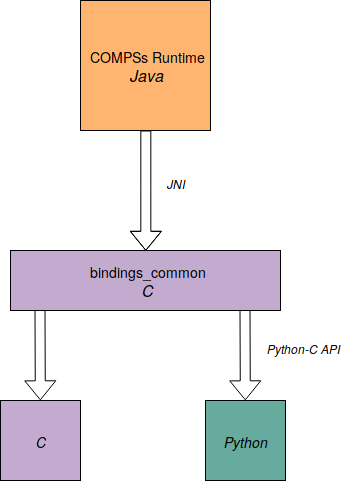
\includegraphics[scale=0.6]{estructuraBindings.png}
    \label{fig:estructura_bindings}
\end{figure}

\subsection{Modelo de ejecución en el binding C/C++}
\label{sec:bindings}

\textit{C} y \textit{C++} son lenguajes de programación compilados, esto quiere decir que necesitamos un segundo programa llamado compilador que procese nuestro programa y genere un fichero que nuestro ordenador pueda ejecutar, a este proceso se le llama compilar y al fichero generado, binario. De esta manera, para poder obtener el modelo de ejecución introducido en la sección \ref{modeloejecucion}, necesitaremos compilar dos binarios, uno para el \textit{master} y otro para los \textit{workers}.
\par\bigskip

\begin{comment}
La aplicación que desarrolla el usuario, \textit{a priori} no envía las tareas a ejecutar ni las dependencias entre estas, no gestiona el \textit{runtime}, pero es desarrollada siguiendo unas directrices que nos permitirán generar código que sí gestione todo lo que es necesario con tal de que la aplicación se distribuya correctamente. 
\end{comment}

La aplicación que desarrolle el usuario, tiene que ser transparente al \textit{runtime}, para conseguirlo tan sólo se necesita una interfaz indicando las tareas a detectar al ejecutar la aplicación. Entonces, una vez compilemos la aplicación de COMPSs en C/C++, se generará automáticamente (a partir de ahora \textit{autogenerar}) código para las tareas, que gestionarán la comunicación con el \textit{runtime}.
\smallskip
La siguiente imagen describe de manera visual cómo se compila una aplicación. 

\begin{figure}[H]
    \centering 
    \caption{Proceso de compilación de una aplicación COMPSs C/C++.}
    %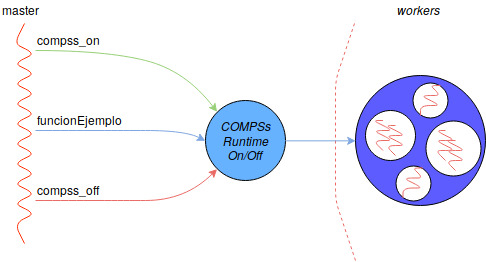
\includegraphics[width=\textwidth]{sta-masterworker.jpg}
    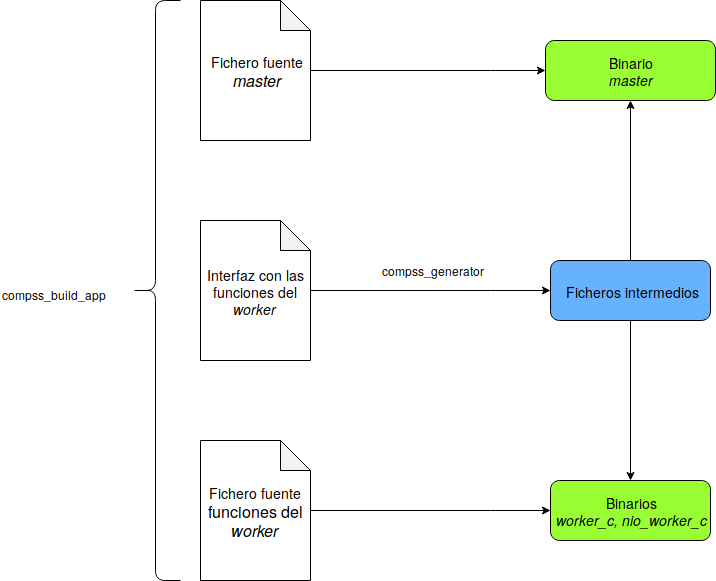
\includegraphics[scale=0.5]{workflowCompilado.png}
    \label{fig:workflowcompilado}
\end{figure}

\par\bigskip
Para facilitar el compilado de la aplicación se utiliza el script \textit{compss\_build\_app}, y para hacer la generación de código a partir de la interfaz, el binario \textit{compss\_generator}.
La aplicación una vez desarrollada por el usuario, compilada sin \textit{COMPSs} por el medio también funcionaría, pero sencillamente las tareas serían ejecutadas \textit{in situ} en el \textit{master}.  Lo que pretendemos hacer al introducir \textit{COMPSs} es que el \textit{master}, en vez de ejecutar la tarea, comunique al \textit{runtime} que se debe ejecutar una tarea, y este se encargue de ejecutarla en un \textit{worker}, todo evidentemente, de manera transparente al usuario.
\par\bigskip

\bigskip
En la figura \ref{fig:workflowcompilado} veíamos la caja negra de ficheros intermedios, estos ficheros son el \textit{stubs} y \textit{executor} (siempre del estilo, \textit{ejemplo-stubs.cc} y \textit{ejemplo-executor.cc} donde ejemplo es el nombre de la aplicación compilada). El fichero \textit{stubs} corresponde con la parte del \textit{master} que se encargará de comunicarse con el \textit{runtime} para registrar la tarea. Esto lo consigue implementando las funciones de las tareas con el código para gestionar su registro, es decir, sustituyendo el código que sería propio de la ejecución de cada tarea por un código para efectuar el registro en el \textit{runtime}. Una vez registrada la tarea, eventualmente el \textit{runtime} designará a un \textit{worker} a ejecutarla. El \textit{worker} recibirá la tarea que debe ejecutar, los datos necesarios y más parámetros, el \textit{executor} ha sido \textit{autogenerado} con el código principal de la aplicación, por lo que conoce como gestionar los datos y parámetros recibidos para ejecutar la tarea pertinente. 

\begin{comment}
\begin{figure}[H]
    \centering  
    \caption{Registro y ejecución de tareas en una aplicación COMPSs C/C++.}
    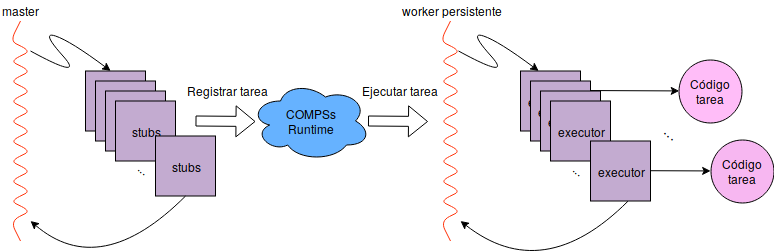
\includegraphics[scale=0.6]{stubs-executor.png}
    \label{fig:stubs-executor}
\end{figure}

La imagen anterior muestra las llamadas a funciones pertinentes a \textit{stubs} que contienen el código para registrar las tareas en el \textit{runtime}, la eventual ejecución de las tareas registradas en los \textit{workers} que haya disponibles y como toma parte su ejecución mediante el \textit{executor}. Ahora que sabemos como se estructura un \textit{binding}, y en concreto, como funciona el de \textit{C/C++}, el siguiente paso es estudiar el funcionamiento de \textit{OmpSs-2}.

%\subsection{Conceptos básicos de OmpSs-2}

\subsubsection{Mercurium}

\textit{Mercurium} es el encargado de compilar una aplicación de \textit{OmpSs-2} y hacer que las directivas insertadas en el código tengan efecto sobre este. De manera superficial, lo que hace es añadir código para gestionar el \textit{runtime}, encender el \textit{runtime}, añadir las tareas, notificar las dependencias y un largo etcétera. 

\subsubsection{Nanos6}

\todo{Pensar algo}
\end{comment}

\subsection{Modo librería: nanos6\_spawn\_function \label{spawnfunction}}

En la sección \ref{sec:bindings} dimos una visión más interna y propia de desarrollador del \textit{binding} de \textit{C/C++}. Sobre \textit{OmpSs-2} necesitamos saber, como se desarrolla una aplicación, en concreto con el modo librería.
\medskip

Esta funcionalidad, nos permite registrar una tarea en el \textit{runtime} de \textit{OmpSs-2} de manera asíncrona, con lo cuál podremos brindar a cada tarea y sus sucesoras un entorno aislado del resto. Gracias a esto, conseguiremos arreglar el problema con la migración de \texit{threads}, planteado en la sección \ref{compssompss}. \smallskip

\begin{lstlisting}[caption={Definición de la función nanos6\_spawn\_function.},captionpos=b, label={lst:nanos6spawn}, language=C++]
void nanos6_spawn_function(
   void (*function)(void *), 
   void *args,
   void (*completion_callback)(void *), 
   void *completion_args, 
   char const *label
);
\end{lstlisting}

La anterior imagen muestra la definición de la función que nos permitirá registrar una función \textbf{function} con argumentos \textbf{args} en el \textit{runtime}. Una vez ejecutada la función registrada como tarea, se ejecutará la función \textbf{completion\_callback} con argumentos \textbf{completion\_args} (mecanismo conocido como \textit{callback}, de ahí el nombre), el argumento de la función \textit{label} sirve para etiquetar la tarea con el nombre que contenga.

\subsubsection{Ejemplo}

Con tal de entender como funciona un programa que utilice el modo librería, vamos a ver un ejemplo sencillo. Este programa de ejemplo, hará \textit{spawn} de una función y dentro de ésta se generarán tareas con dependencias entre ellas. \smallskip

\begin{lstlisting} [caption={Función a ser registrada como tarea.},captionpos=b, label={lst:nanos6\_ejemplo}, language=C++]
 int nanos6_ejemplo(int* a) {

    int local_a;

    #pragma oss task shared(local_a) out(local_a) 
    {
        local_a = a[0];
    }

    #pragma oss task shared(local_a) inout(local_a)
    {
        local_a = local_a * 4;
    }

    #pragma oss taskwait

    return local_a;
}
\end{lstlisting}

En la imagen podemos ver la función \textbf{nanos6\_ejemplo}, ésta tiene como parámetro un puntero a enteros \textbf{a} y retorna un valor del tipo \textbf{int}. La función será registrada como tarea desde otro fichero. El cálculo que se realiza en la función no tiene la menor importancia, es solo un \textbf{ejemplo}. \medskip

Por supuesto, esta función será compilada con \textit{Mercurium}, si no fuera el caso, la función se ejecutaría correctamente pero no se generarían las tareas de dentro de la función, por lo cuál la ejecución sería secuencial. 

\begin{lstlisting} [caption={Gestión del modo librería desde el main.},captionpos=b, label={lst:library-main}, language=C++]
    char const *error = nanos6_library_mode_init();
    if (error != NULL)
    {
        fprintf(stderr, "Error initializing Nanos6: %s\n", error);
        return 1;
    }

    condition_variable_t cond_var = COND_VAR_INIT;

    ejemplo_wrapper_args_t args;

    int A = 1;
    args.array = &A;
    
    nanos6_spawn_function(ejemplo_wrapper, &args, 
    condition_variable_callback, &cond_var, 
    "spawned ejemplo");

    wait_condition_variable(&cond_var);

    printf("%li\n", args.ret);

    nanos6_shutdown();

\end{lstlisting}

Las funciones \textit{nanos6\_library\_mode\_init()} y \textit{nanos6\_shutdown()} efectúan respectivamente el encendido y apagado del \textit{runtime}, el código que vemos entre estas dos llamadas es el correspondiente para registrar una función como tarea utilizando el modo librería. Dado que la función nanos6\_spawn\_function espera como un puntero los parámetros a pasar a la función, se deben incluir todos dentro de una estructura que los pueda contener, el \textit{struct} \textit{ejemplo\_wrapper\_args\_t} tiene los campos \textbf{a} y \textbf{ret} que corresponden al parámetro de la función \textit{nanos6\_ejemplo} y valor de retorno de ésta.

\bigskip
Un detalle que no se ha comentado es que la ejecución de este código será efectuada por \textit{pthreads}, el estándar \textit{POSIX} de \textit{threads}. Dado que la ejecución de la tarea tendrá lugar de manera \textbf{asíncrona} es necesario un mecanismo de sincronización, la implementación de \textit{threads} que utilizamos (y por tanto los mecanismos de sincronización dependerán de estos) es la explicada en el apéndice \ref{appendix:pthread}.

\bigskip

Como es necesario utilizar una estructura auxiliar para pasar los parámetros mediante un puntero, necesitaremos también una función intermedia con la cuál llamar a la función que realmente queremos registrar como tarea. Habitualmente a este tipo de funciones intermedias se les llama \textit{wrapper}. En la siguiente imagen veremos la función que actúa como \textit{wrapper} de la función \textit{nanos6\_ejemplo}. \smallskip

\begin{lstlisting} [caption={Wrapper de la función nanos6\_ejemplo.},captionpos=b, label={lst:library-wrapper}, language=C++]
 void ejemplo_wrapper(void *untyped_arg)
{
    ejemplo_wrapper_args_t *args = 
        (ejemplo_wrapper_args_t *) untyped_arg;
    args->ret = nanos6_ejemplo(args->a);
}
\end{lstlisting}

El puntero de tipo \textit{void} puede contener cualquier tipo de estructura, aprovechando que sabemos que únicamente deberá contener el tipo \textit{ejemplo\_wrapper\_args\_t} se hace un \textit{cast} para interpretarlo como la estructura deseada. Se asigna \textbf{ret} al valor de retorno y se pasa \textbf{a} como parámetro.

\todo{faltan detalles de compilado...}

\subsection{Integración}

Ahora que tenemos claro el funcionamiento de ambas partes, podemos plantear un prototipo de la integración e implementarlo. Está claro que \textit{OmpSs-2} tomará parte únicamente en los nodos del tipo \textit{worker}, ya que es dónde realmente se ejecutarán las tareas detectadas por el \textit{master}. 
\par\medskip

En el ejemplo para utilizar el modo librería \ref{spawnfunction}, aprendimos como activar el \textit{runtime} de \textit{OmpSs-2} en este modo y como ejecutar las tareas, por lo que bastará con activarlo en los \textit{workers} (persistente y no persistente) y modificar la generación del código \textit{executor} (queremos hacerlo en el \textit{worker}) para generar la misma estructura del ejemplo en cada tarea de la interfaz de la aplicación.
\par\medskip
Entonces, con la activación de \textit{OmpSs-2} en los nodos \textit{worker} conseguiremos la siguiente estructura y modelo de ejecución.

\begin{figure}[H]
    \centering 
    \caption{Estructura y modelo de ejecución master-worker de la integración COMPSs+OmpSs-2}
    %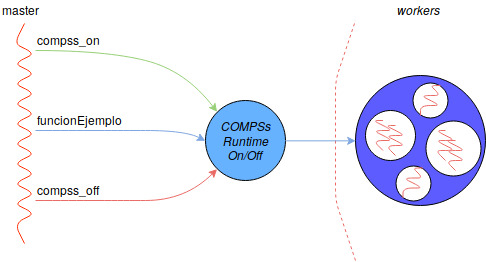
\includegraphics[width=\textwidth]{sta-masterworker.jpg}
    \includegraphics[scale=0.5]{compss2rt.png}
    \label{fig:compssompssrt}
\end{figure}

Durante la ejecución del programa principal se irá generando un grafo con las tareas que se deben ejecutar, eventualmente cada una de estas será enviada a un nodo \textit{worker} (en la figura tan sólo aparece uno, pero podrían ser más) y este ejecutará la tarea de \textit{COMPSs} en forma de tarea de \textit{OmpSs-2}.
La ejecución de las tareas de \textit{OmpSs-2} generará otro grafo, dónde figurarán tanto las tareas que han sido creadas mediante el mecanismo de \textit{spawn} como las que puedan ser creadas dentro de las anteriores, y finalmente las tareas de este grafo serán ejecutadas.

\subsubsection{Encendido y apagado del modo librería}

\todo{nio worker c y worker c}

\subsubsection{Generación del código de cada tarea}

\todo{spawn en sí}

\subsubsection{Modificaciones en la compilación actual}

\todo{modificacion de los scripts, autotools, etc}

\subsubsection{Tipo enum y cabeceras en la interfaz}

\todo{Añadido del tipo enum y el include de las cabeceras}

\section{Aplicación COMPSs+OmpSs-2}



\section{Estudio del rendimiento}

































\chapter{Evaluación}
\label{sec:estudiorend}

En este capítulo describiremos las aplicaciones descritas para evaluar la integración \textit{COMPSs+OmpSs-2}, los entornos donde haremos la evaluación y los resultados de esta.  

\section{Aplicaciones}
\subsection{K-Means}

\textit{K-Means} es un algoritmo utilizado para hacer \textit{clustering} sobre un grupo de datos, es decir, agrupar los datos en \textit{clusters}. Cada dato pertenece al \textit{cluster} cuyo centro está en la distancia mínima, si no fuera así pertenecería a otro \textit{cluster}. Se inicializan \textit{clusters} con centros escogidos de manera aleatoria y se comparan las distancias a todos los \textit{clusters} y se determina a cual pertenece cada dato (siempre al centro más cercano), una vez hecho esto se vuelve a calcular el centro de cada \textit{cluster}, todo este proceso conforma una iteración de \textit{K-Means}, habitualmente se itera hasta que converge, esto es que la distancia entre los centros asignados en dos interaciones consecutivas de cada \textit{cluster} es cercana a 0.

\begin{figure}[h]
	\centering 
	\caption{Grafo de dependencias entre tareas de K-Means.}
	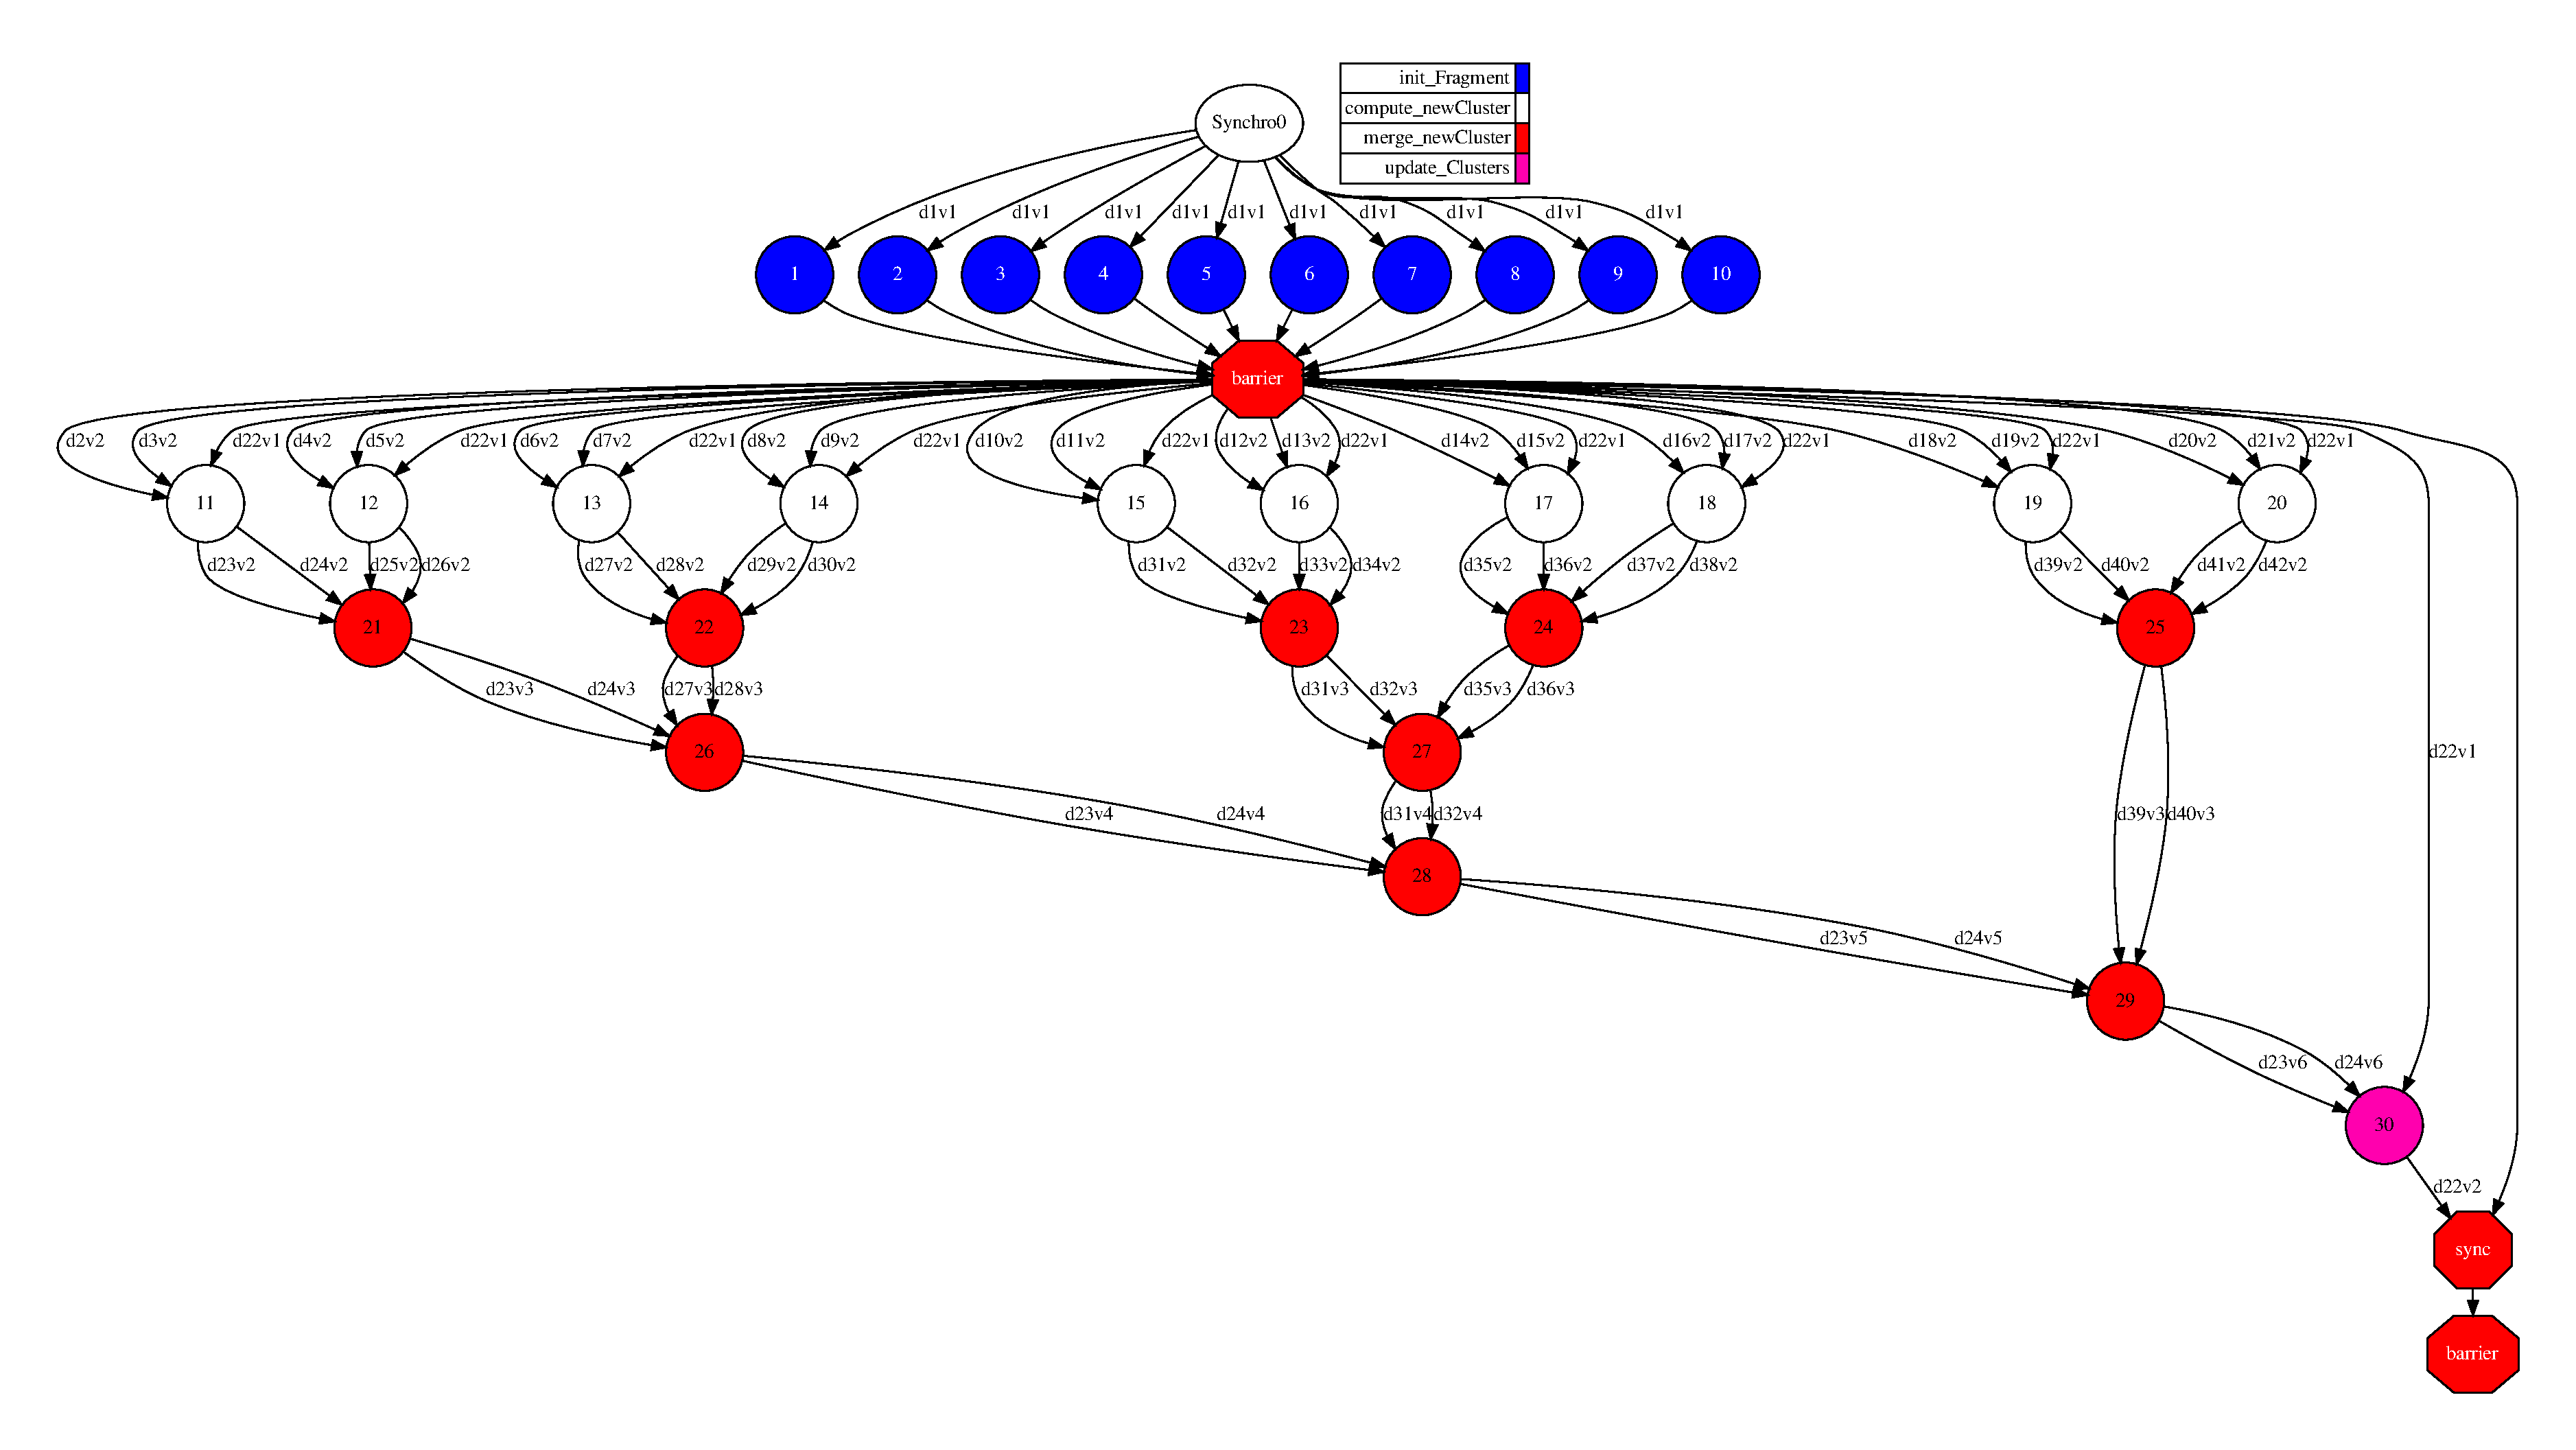
\includegraphics[scale=0.2]{grafo_kmeans.pdf}
	\label{fig:grafokmeans}
\end{figure}

Tal y como hemos desarrollado la aplicación tiene 4 tareas, que son \textit{init\_Fragment}, \textit{compute\_newCluster} (tiene una implementación en CPU y otra en GPU), \textit{merge\_newCluster}, \textit{update\_Clusters}. La imagen \ref{fig:grafokmeans} muestra un grafo de dependencias de una ejecución de \textit{K-Means} donde el número de \textit{clusters} a formar es 25 y se efectúa una única iteración. Para no sobrecargar este apartado se incluye en el apéndice \ref{sec:codigokmeans} la interfaz y el programa principal de la aplicación.

\subsection{Cholesky}

\textit{Cholesky} es un método de descomposición aplicable cuando la matriz es simétrica definida positiva, entonces esta puede ser descompuesta como el producto de una matriz triangular inferior y su traspuesta. El método \textit{Cholesky} se utiliza para resolver sistemas de ecuaciones lineales, es similar a la descomposición \textit{LU} y es el doble de eficiente.
\par\bigskip
La aplicación ha sido desarrollada utilizando una librería para operaciones de algebra lineal programada en \textit{C} con \textit{OmpSs} y \textit{OmpSs-2}, esta librería es \textit{LASs}\footnote{https://pm.bsc.es/mathlibs/lass} (\textit{Linear Algebra routines on OmpSs}). Las funciones que implementa \textit{LASs} serán utilizadas como tareas a nivel de \textit{COMPSs} y después una vez ejecutadas harán uso de \textit{OmpSs-2}, por lo que realmente desarrollar una aplicación utilizando una librería externa es muy sencillo.
\par\bigskip
Tiene 5 tareas, \textit{generate\_block}, \textit{ddss\_dpotrf}, \textit{ddss\_dtrsm}, \textit{ddss\_dgemm}, \textit{ddss\_dsyrk}, \textit{generate\_block} se utiliza para generar los bloques de manera distribuida (así el \textit{master} no tiene reservar memoria para toda la matriz, que podría ser muy grande), las otras 4 tareas son operaciones de algebra lineal que utilizadas de la forma correcta aplicarán el método de descomposición de \textit{Cholesky}.
En el apéndice \ref{sec:codigocholesky} se encuentra la interfaz y el programa principal de la aplicación. 

\begin{figure}[h]
	\centering 
	\caption{Grafo de dependencias entre tareas de Cholesky.}
	\includegraphics[scale=0.07]{grafo_cholesky.pdf}
	\label{fig:grafocholesky}
\end{figure}

La imagen \ref{fig:grafocholesky} muestra un grafo de dependencias de la aplicación \textit{Cholesky} con una matriz de 64 bloques con 4096x4096 elementos cada uno. 

\section{Entornos para el estudio}

Para la realización del estudio del rendimiento se han utilizado dos máquinas que el \textit{Barcelona Supercomputing Center} pone a nuestra disposición, que son \textit{CTE-Power} y \textit{MareNostrum4}.

\subsection{CTE-Power}
\label{sec:power}

\textit{CTE-Power} es un \textit{cluster} basado en la tecnología de procesadores \textit{IBM} \textit{Power9}. Tiene 2 nodos de \textit{login}, son los nodos desde donde operan los usuarios y 52 nodos de cómputo. 
\par\smallskip
Cada nodo tiene los siguientes componentes:
\par\smallskip
\begin{itemize}
	\item 2 x \textit{IBM Power9 8335-GTH} @ 2.4GHz (3.0GHz en modo turbo), cada procesador con 20 cores cada uno con 4 \textit{threads}.
	\item 512GB de memoria organizada en 16 \textit{dimms} de 32GB @ 2666MHz.
	\item 4 x \textit{NVIDIA} V100 con 16GB \textit{HBM2}.
	\item 2 x SSD que proporcionan 1.9TB de almacenaje local.
	\item 2 x \textit{NVM Express} 3.2TB.
	\item Interfaz de red \textit{Mellanox}.
	\item Sistema de ficheros GPFS a través de fibra a 10GBit.
\end{itemize}

Nosotros utilizaremos tan sólo 10 nodos, por lo que tendremos a nuestra disposición en la mayor ejecución 1600 CPUs y 40 GPUs \textit{NVIDIA V100}. 

\subsection{MareNostrum4}
\label{sec:mare}

\textit{MareNostrum4} es un supercomputador basado en la tecnología de procesadores \textit{Intel Xeon Platinum} de la generación \textit{Skylake}. Tiene 5 nodos de \textit{login} y 3.456 nodos de cómputo.
\par\smallskip
Cada nodo tiene los siguientes componentes:
\par\smallskip
\begin{itemize}
	\item 2 x \textit{Intel Xeon Platinum 8160 @ 2.10GHz} con 24 cores.
	\item Hay nodos con distintos tipos de memoria:
		\subitem 1,88 GB/core de memoria. %organizada en 12 \textit{dimms} de 8GB @ 2667MHz.
		\subitem 7,93 GB/Core de memoria.
	\item Un SSD que proporciona 200 GB de almacenaje local.
	\item 100 Gbit/s \textit{Intel Omni-Path HFI Silicon 100 Series PCI-E adapter}.
	\item 10 Gbit \textit{Ethernet}.
\end{itemize}

Igual que con \textit{CTE-Power} tan sólo utilizaremos 10  nodos, por lo tanto tendremos en la mayor ejecución 480 CPUs.

\section{K-Means}

La evaluación con \textit{K-Means} ha consistido en hacer un test de \textit{strong scaling}, que consiste en ejecutar la aplicación con un tamaño de problema fijo y aumentar el número de recursos de cómputo, y otro de \textit{weak scaling} donde aumentaremos de manera proporcional el tamaño del problema y los recursos de cómputo. En el apartado \ref{sec:power} describimos la máquina que utilizamos en estos test, haremos uso de todas las \textit{CPUs} y \textit{GPUs} de cada nodo.

\subsection{Strong scaling}

La imagen \ref{fig:sc-time} muestra una gráfica que tiene en el eje vertical el tiempo y en el horizontal el número de nodos. El tamaño del problema que se ha utilizado es de 400 fragmentos de 50 dimensiones y 200000 puntos cada uno, el número de \textit{clusters} a formar es 50 y se efectúan 5 iteraciones. Se han tomado 10 muestras de cada ejecución, la línea azul muestra la media de las muestras para el mismo número de nodos, la de color naranja muestra el tiempo ideal que debería tardar según el número de nodos. En cada punto de la línea azul se muestra la diferencia entre el máximo valor y el mínimo que se han tomado en las muestras.

\begin{figure}[H]
	\centering 
	\caption{Tiempo de ejecución al aumentar el número de recursos.}
	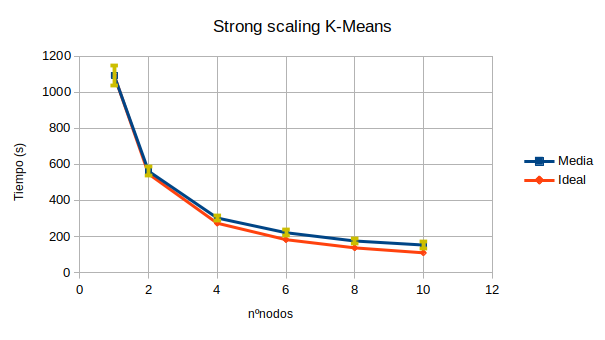
\includegraphics[scale=0.8]{estudio/KMeans/sc/kmeans-sc-time.png}
	\label{fig:sc-time}
\end{figure}

Es bueno que la línea azul sea lo más parecida a la línea naranja, eso nos indicaría que la aplicación escala perfectamente, ya que cada vez que aumentamos los recursos el tiempo de ejecución se reduciría proporcionalmente. La imagen \ref{fig:sc-speedup} muestra la misma información que \ref{fig:sc-time} dispuesta en forma de ganancia, se puede ver que se comporta bien hasta que en los 6 nodos empieza a dejar de acercarse al ideal.

\begin{figure}[H]
	\centering 
	\caption{Ganancia al aumentar el número de recursos.}
	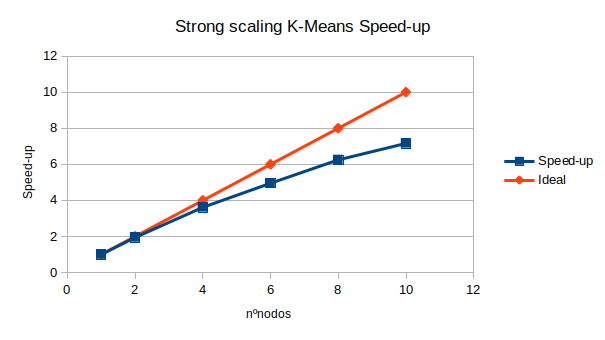
\includegraphics[scale=0.8]{estudio/KMeans/sc/kmeans-sc-speedup.png}
	\label{fig:sc-speedup}
\end{figure}

\subsection{Weak scaling}

En un test de \textit{weak scaling}, esperamos que los tiempos de ejecución sean siempre los mismos, ya que el tamaño del problema es siempre proporcional a los recursos de cómputo. Esto sería perfecto pero hay que efectuar comunicación entre nodos y gestionar todo el sistema, por lo que no podemos mantener este escenario ideal. La imagen \ref{fig:wc-effic} muestra cómo al aumentar el número de nodos la eficiencia baja del ideal (que el tiempo de ejecución sea siempre el mismo), pero se mantiene alrededor del mismo valor a partir de los 6 nodos.

\begin{figure}[H]
	\centering 
	\caption{Eficiencia al mantener proporcional el tamaño del problema y el número de recursos.}
	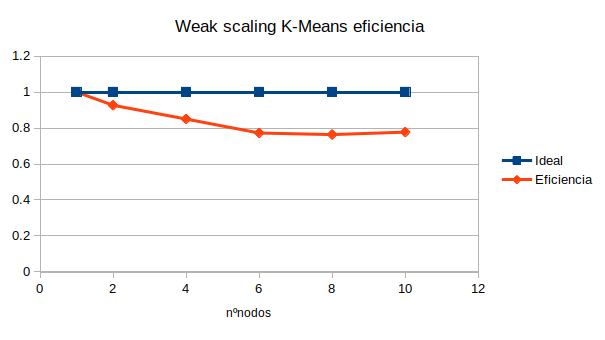
\includegraphics[scale=0.8]{estudio/KMeans/wc/kmeans-wc-efficiency.png}
	\label{fig:wc-effic}
\end{figure}

\section{Cholesky}











\appendixpage
\appendix


\begin{landscape}
\appendixpage
\appendix
\section{Planificación y diagrama de Gantt correspondiente}

\begin{figure}[H]
    \centering 
    \caption{Tareas definidas para el diagrama de Gantt.}
    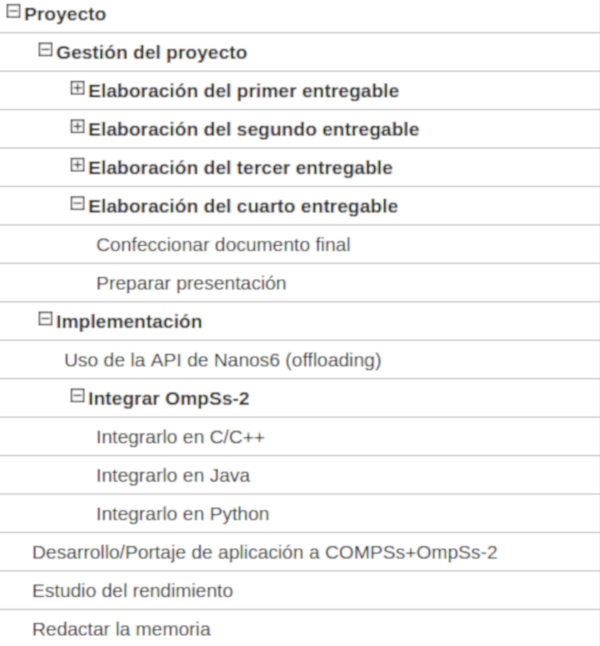
\includegraphics[scale=2.5]{ganttProyecto.png}
    \label{fig:gantt_tareas}
\end{figure}

\begin{figure}[H]
    \centering 
    \caption{Diagrama de Gantt del proyecto.}
    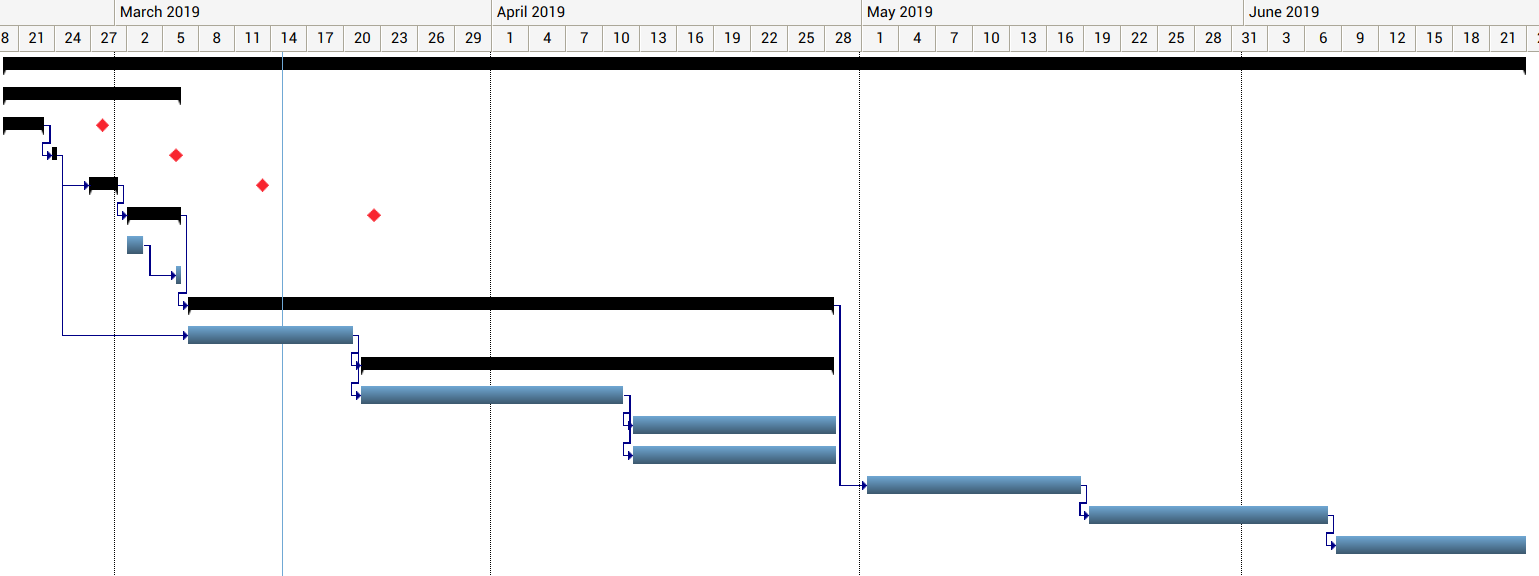
\includegraphics[scale=2]{diagramaGantt.png}
    \label{fig:diagrama_gantt}
\end{figure}
\end{landscape}

\externaldocument{technical_work/ompss-2-integration.tex}

\section{Pthreads y mecanismos de sincronización}
\label{appendix:pthread}

En este apéndice se introduce superficialmente qué es un \textit{Pthread} y se hace hincapié en el mecanismo utilizado para la sincronización con las tareas registradas en \textit{Nanos6} con el modo librería introducido en la sección \ref{spawnfunction}
\bigskip

Históricamente los \textit{threads} se han implementado por cada fabricante o empresa, de una manera específica, complicando la portabilidad entre plataformas. Los \textit{Pthreads} nos proveen un estándar con la intención de que sea utilizado por la mayoría de máquinas. En todos los sistemas operativos del tipo \textit{UNIX} se implementan los \textit{threads} con el estándar \textit{IEEE POSIX 1003.1c}, y se les llama \textit{POSIX threads} o \textit{Pthreads}. El manual se puede encontrar en internet, y explica de lo más básico a lo más avanzado \cite{barney2009posix}. \todo{la cita ?}
\bigskip

Requerimos de un mecanismo de sincronización por que la función que se registra como tarea la ejecuta un \textit{thread} diferente al que la registra. 

\begin{figure}[H]
    \centering 
    \caption{Mecanismo de sincronización abstracto.}
    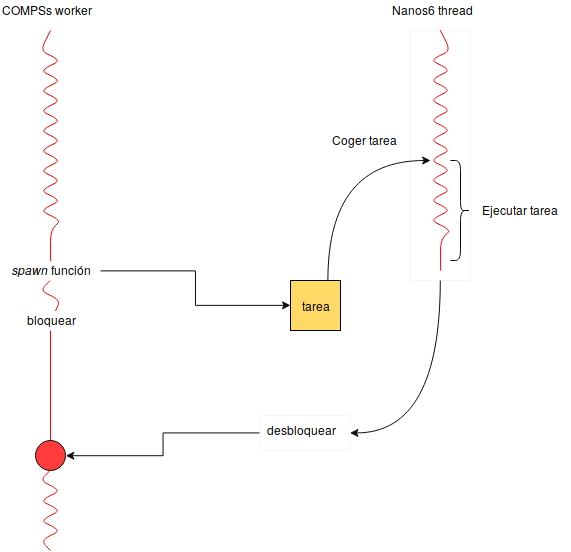
\includegraphics[scale=0.6]{spawn_sync.png}
    \label{fig:spawn_sync}
\end{figure}

En la figura anterior se muestran dos \textit{threads}, uno que registra una tarea y otro que espera a poder ejecutar alguna tarea. El primer \textit{thread} una vez haya registrado la tarea procederá a bloquearse, el segundo cuando acabe de ejecutar la tarea registrada, ejecutará un \textit{callback} donde desbloquearemos al primer \textit{thread}. \bigskip

El mecanismo abstracto es sencillo, pero la implementación real depende de los \textit{Pthreads}. Las estructuras utilizadas para realizar la sincronización son \texit{mutexes} y \textit{condition variables}. Un \textit{mutex} es una estructura que sirve para definir regiones de exclusión mútua mediante métodos de adquisición y liberación de la región, en este mecanismo se utilizan tan sólo por que son necesarios para utilizar \textit{condition variables}. Las \textit{condition variables} nos permiten que un \textit{thread} espere a un evento de manera no bloqueante, si no, habría que hacer \textit{polling} y consumir tiempo de cómputo inútilmente.
\bigskip

Será con las funciones \textit{pthread\_cond\_wait(pthread\_cond\_t * cond, pthread\_mutex\_t * mutex)} y \textit{pthread\_cond\_signal(pthread\_cond\_t * cond)} con las que respectivamente bloqueemos al primer \textit{thread} después de registrar la tarea y lo desbloqueemos al acabar de ejecutarla.
\bigskip

Dado que para utilizar \textit{condition variables} se necesitan \textit{mutexes} y se recomienda utilizar una variable auxiliar para evitar abrazos mortales (en el caso de que, el segundo \textit{thread} ya ha intentado desbloquear al primero, pero este aún no se había bloquedao, cuando se bloquee, se bloqueará para siempre), se crea una estructura de datos para contener todas estas variables llamada \textit{condition\_variable\_t}.

\smallskip

\begin{lstlisting} [caption={Definición de la estructura de datos condition\_variable\_t.},captionpos=b, label={lst:wait-condition}, language=C++]
typedef struct {
    pthread_mutex_t _mutex;
    pthread_cond_t _cond;
    int _signaled;
} condition_variable_t;
\end{lstlisting}

\smallskip

\begin{lstlisting} [caption={Función wait\_condition\_variable},captionpos=b, label={lst:wait-condition}, language=C++]
void wait_condition_variable(condition_variable_t *cond_var)
{
    pthread_mutex_lock(&cond_var->_mutex);
    while (cond_var->_signaled == 0) {
        pthread_cond_wait(&cond_var->_cond, &cond_var->_mutex);
    }
    pthread_mutex_unlock(&cond_var->_mutex);
}
\end{lstlisting}

En la imagen \ref{lst:library-main} se utiliza la función \textit{wait\_condition\_variable(&cond\_var)}, la llamada a  \textit{pthread\_cond\_wait} está dentro de una región crítica para prevenir que nadie más se bloquee sobre la misma \textit{condition variable} y esta se encuentra dentro de un \textit{while} por que puede ocurrir que el \textit{thread} se desbloquee sin haber sido desbloqueado por otro \textit{thread}, la variable \textit{cond\_var->\_signaled} será 0 hasta que el \textit{thread} que produzca el desbloqueo lo modifique, así garantizaremos que el desbloqueo es intencionado.
\smallskip

\begin{lstlisting} [caption={Callback de la tarea registrada},captionpos=b, label={lst:signal-condition}, language=C++]
void condition_variable_callback(void *untyped_arg)
{
    condition_variable_t *cond_var = (condition_variable_t *) untyped_arg;

    pthread_mutex_lock(&cond_var->_mutex);
    cond_var->_signaled = 1;
    pthread_cond_signal(&cond_var->_cond);
    pthread_mutex_unlock(&cond_var->_mutex);
}
\end{lstlisting}

La imagen anterior muestra el \textit{callback} que se ejecuta al finalizar la ejecución de la tarea, modifica el valor de la variable \textit{cond\_var->\_signaled} y efectúa un \textit{pthread\_cond\_signal} para despertar al primer \textit{thread}.












%https://www.gnu.org/software/automake/manual/html_node/Autotools-Introduction.html

\section{Autotools}
\label{appendix:autotools}
 
\textit{Autotools} es un conjunto de herramientas que pretenden facilitar la difícil tarea de crear codigo fuente portable entre plataformas del tipo \textit{UNIX} de manera sencilla, es decir, de poder compilar el código fuente de una aplicación en en varias plataformas implicando un esfuerzo pequeño (para el usuario). \textit{Autotools} forma parte de la \textit{GNU Toolchain} desarrollado por el \textit{GNU Project\footnote{https://www.gnu.org/gnu/thegnuproject.html}}.


\newpage

\bibliographystyle{plain}
\bibliography{bibliography.bib}
\nocite{*}
\end{document}
\printbibliography
